\documentclass{article}
\usepackage{geometry}
\usepackage{hyperref}
\usepackage{pdfpages}

\title {Khidmat: Teaching Programming on Scratch}

\author{
  Syed Ahsan Ahmed\\ sa02908
}
\date{}  

\begin{document}
\maketitle

This project is to teach programming concepts on Scrach using Drag-Drop programming to underpriviliged students at Fixit School.

Fixit School is a non-profit organization and an initiative by FIXIT to provide free education to the underprivileged children of Pakistan. Students of all ages are taught fundamental subjects, such as English , Maths, Science, Urdu, Islamiat. 

Fixit School teaches its students the fundamental subjects of Science and Literature. It was felt that the students should be taught basic programming concepts on Scratch (Drag-Drop programming) that they can use in the lives ahead and progress in the field of Computer Science.

We will be teaching the students 2 hours daily on Fixit School's premises under the supervision of their Admission Manager. The goal is to teach them the basic programming concepts and make them capable of building their own games using drag-n-drop programming on Scratch.

\newpage
\section*{Week 1: 14--18 May, 2018}

We spent this week teaching the students for-loops, and if-statements. Board games, two 'Hour of Code' and the EDVON software, were used to teach these concepts.

\begin{tabular}{|l|l|l|l|}
  \hline
  Item  & Activity & Time & ID \\\hline\hline
  1 & Board games & 2.5 hrs & sa02908 \\\hline
  2 & Hour of Code practice (2 sessions) & 2.5 hrs & sa02908 \\\hline
  3 & For loops & 2.5 hrs & sa02908 \\\hline
  4 & If Statements & 2.5 hrs & sa02908 \\\hline
\end{tabular}

The total time spent on the Khidmat this week is as follows.

\begin{tabular}{|l|l|}
  \hline
  ID & Total Hours\\\hline\hline
  sa02908 & 10 hours\\\hline
\end{tabular}

% week 2

\newpage 
\section*{Week 2: 21--25 May, 2018}

We spent this week teaching the students while-loops, along with practice on hour of code. Students were also familiarized with EDVON.

\begin{tabular}{|l|l|l|l|}
  \hline
  Item  & Activity & Time & ID \\\hline\hline
  1 & While loops & 2.5 hrs & sa02908 \\\hline
  2 & Hour of Code practice & 2.5 hrs & sa02908 \\\hline
  3 & Edvon Practice (loops) & 5 hrs & sa02908 \\\hline
\end{tabular}

The total time spent on the Khidmat this week is as follows.

\begin{tabular}{|l|l|}
  \hline
  ID & Total Hours\\\hline\hline
  sa02908 & 10 hours\\\hline
\end{tabular}

% week 3

\newpage 
\section*{Week 3: 28 May--1 June, 2018}

We spent this week teaching the students about Events, variables, and the types of variables.

\begin{tabular}{|l|l|l|l|}
  \hline
  Item  & Activity & Time & ID \\\hline\hline
  1 & Events & 2.5 hrs & sa02908 \\\hline
  2 & Variables & 2.5 hrs & sa02908 \\\hline
  3 & Edvon Practice (events) & 5 hrs & sa02908 \\\hline
\end{tabular}

The total time spent on the Khidmat this week is as follows.

\begin{tabular}{|l|l|}
  \hline
  ID & Total Hours\\\hline\hline
  sa02908 & 10 hours\\\hline
\end{tabular}

% week 4

\newpage 
\section*{Week 4: 4--8 June, 2018}

We spent this week giving students extensive hands-on-learning experience and creating games games.

\begin{tabular}{|l|l|l|l|}
  \hline
  Item  & Activity & Time & ID \\\hline\hline
  1 & Edvon Practice (all) & 10 hrs & sa02908 \\\hline
\end{tabular}

The total time spent on the Khidmat this week is as follows.

\begin{tabular}{|l|l|}
  \hline
  ID & Total Hours\\\hline\hline
  sa02908 & 10 hours\\\hline
\end{tabular}

% week 5

\newpage
\section*{Week 1: 11--14 June, 2018}

We spent this week giving students dense hands-on-learning experience and creating games games.

\begin{tabular}{|l|l|l|l|}
  \hline
  Item  & Activity & Time & ID \\\hline\hline
  1 & Edvon Practice (all) & 4 hrs & sa02908 \\\hline
  2 & Exam & 2.5 hrs & sa02908 \\\hline
  3 & Viva & 1.5 & sa02908 \\\hline
\end{tabular}

The total time spent on the Khidmat this week is as follows.

\begin{tabular}{|l|l|}
  \hline
  ID & Total Hours\\\hline\hline
  sa02908 & 8 hours\\\hline
\end{tabular}

\newpage
\section*{Conclusion}

Our project was to teach the students of Fixit School programming on Scratch. We started by teaching them concepts like loops and statements through on-board games and then moved to 'Hour of Code' sessions. After the students had done sufficient practice on it, we moved them to EDVON and familiarised them with its tools. At the end of the classes, students had learned to create their own games on EDVON/Scratch, and had already developed 10+ games, including a multiplayer game.

\newpage

\thispagestyle{empty}
% Show your external supervisor your report, especially the weekly upates; have them sign a printed copy of this page; scan the signed page; and include the scanned page in this document as an image.

\begin{center}
  {\Large\bf Khidmat Completion Form}\\[5pt]
  \small To be completed by the external supervisor.  
\end{center}
\bigskip

\noindent{\it Please use the space below to provide any comments you may have on the students' performance, the Khidmat program, or any other feedback you want to share with Habib University's Khidmat committee. We can also be reached at \href{mailto:khidmat@sse.habib.edu.pk}{khidmat@sse.habib.edu.pk}.}
\vfill

\begin{center}
  \rule{.8\textwidth}{.5pt}
\end{center}
\medskip

% Insert your name below.

I hereby certify that I supervised Syed Ahsan Ahmed for the Khidmat described in this report. Furthermore, that I have read and agree with the weekly updates included in this report. My signature below marks the successful completion of the work undertaken for the Khidmat.\\
\bigskip
\bigskip

\noindent\begin{tabular}{@{}p{.6\textwidth}@{\hspace{.1\textwidth}}p{.3\textwidth}}
  \hrulefill &   \hrulefill \\
  Name and signature & Location and date
\end{tabular}


 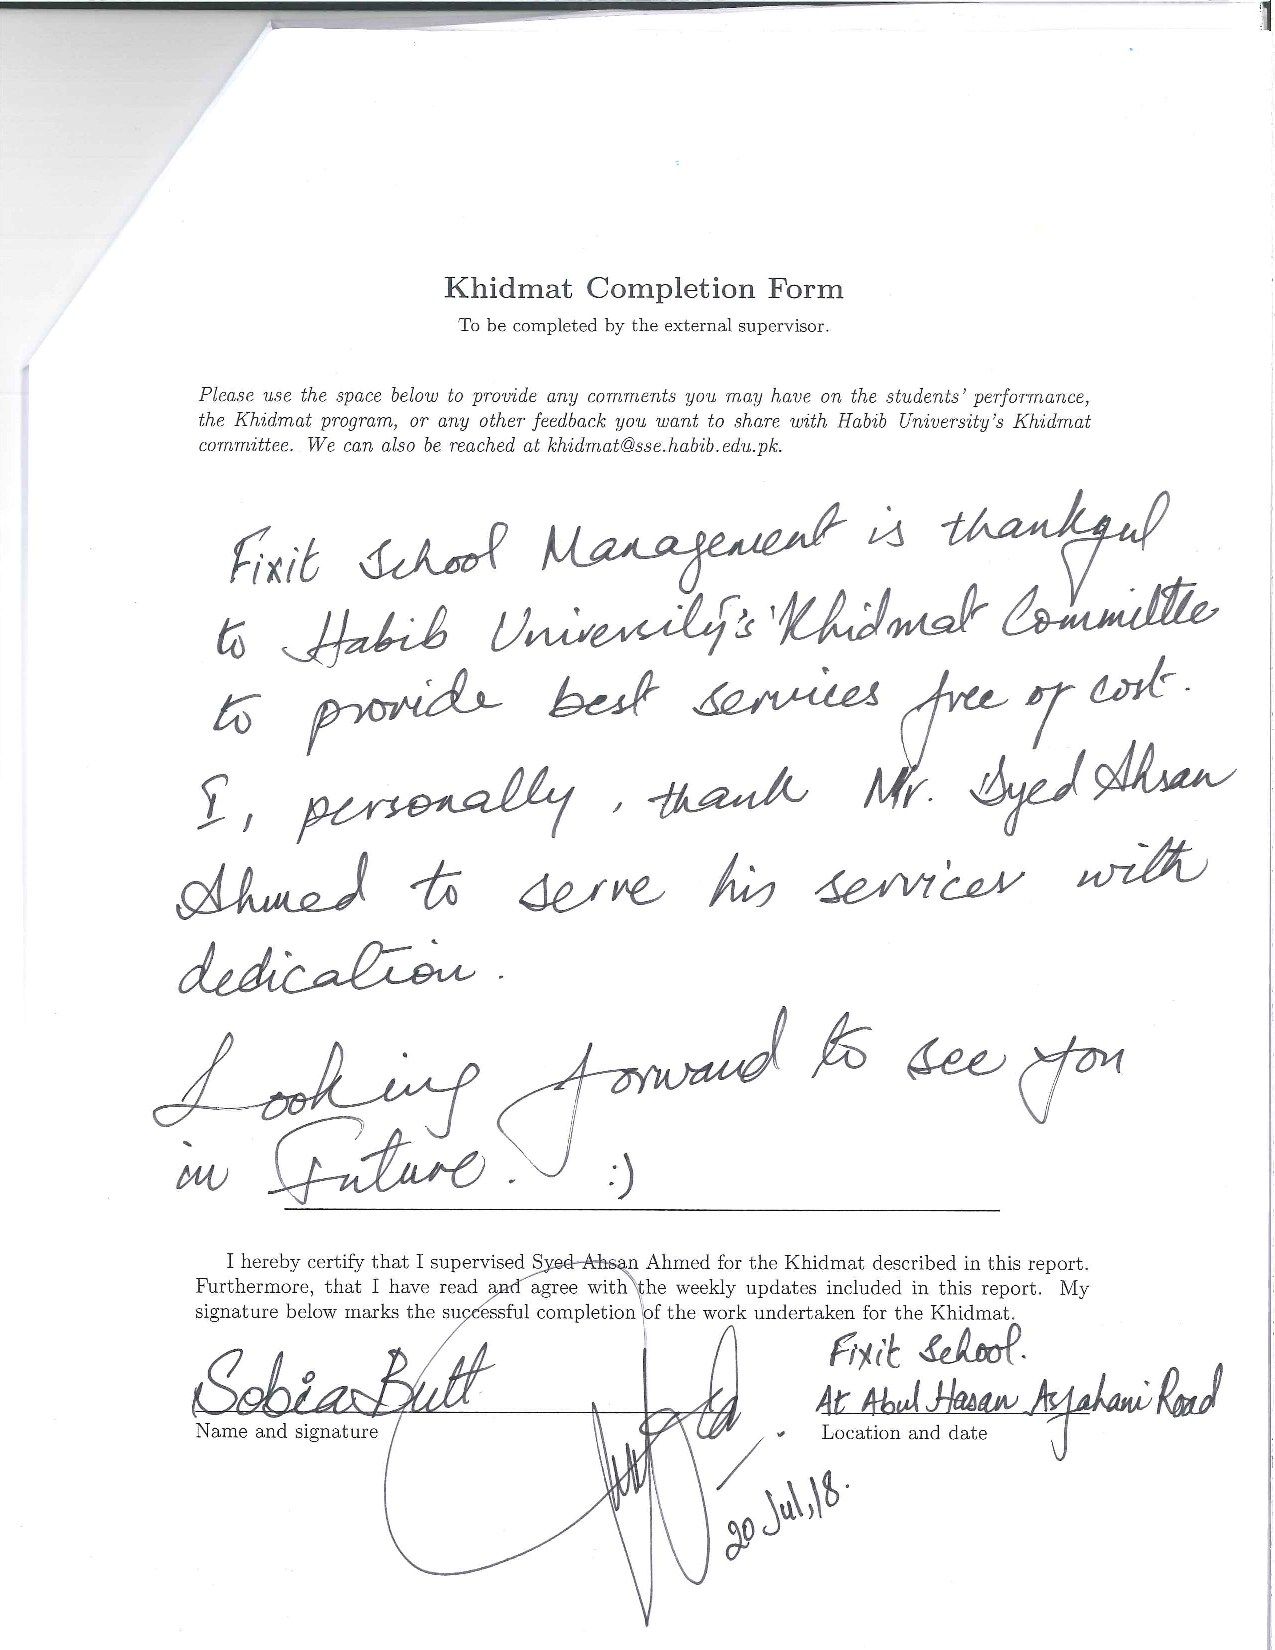
\includepdf[page={1}]{sign.pdf}

\end{document}
